\documentclass[11pt, a4paper]{book}

% {{{ Packages
        \usepackage[margin=1in]{geometry}                           % Margins
          \linespread{1.2}                                          % Increases line spacing
        \usepackage{graphicx}                                       % Image Support
          \graphicspath{ {./images/} }                              % Path to image directory
        \usepackage{color}                                          % Colors for stuff
        \usepackage{soul}                                           % Provides Highlight feature
        \usepackage{fancyhdr}                                       % Fancy Header and footer
        \usepackage{amsmath}                                        % Math support
        \usepackage{amssymb}                                        % Extended symbols for math
        \usepackage{todonotes}                                        % Extended symbols for math
        % \usepackage{etoolbox}                                       % IDK what it does. I just coppied it from stackexchage
        %   \AtBeginEnvironment{align}{\setcounter{equation}{0}}      % resets align counter for each instance
        \usepackage{listings}                                       % Code-snippet support
          \definecolor{dkgreen}{rgb}{0,0.6,0}                     % lst-configs
          \definecolor{gray}{rgb}{0.5,0.5,0.5}
          \definecolor{mauve}{rgb}{0.58,0,0.82}

          \lstset{                                                % lst-format-config
            frame=tb,
            language=Java,
            aboveskip=3mm,
            belowskip=3mm,
            showstringspaces=false,
            columns=flexible,
            basicstyle={\small\ttfamily},
            numbers=none,
            numberstyle=\tiny\color{gray},
            keywordstyle=\color{blue},
            commentstyle=\color{dkgreen},
            stringstyle=\color{mauve},
            breaklines=true,
            breakatwhitespace=true,
            tabsize=3
          }
        \usepackage{caption}                                      % Caption support
        \usepackage[utf8]{inputenc}                               % utf encoding
        \usepackage{hyperref}
          \hypersetup{pdfnewwindow=true, colorlinks=false}
% }}}

% {{{ Footer section
        % Creates footer
        \pagestyle{fancy}%
        \fancyhf{}%
        \lfoot{Swapnil}%
        \cfoot{iamb4uc.xyz}%
        \rfoot{Page \thepage}%
        \renewcommand{\headrulewidth}{0pt}% Line at the head invisible
        \renewcommand{\footrulewidth}{0.4pt}% Line at the footer visible

        % Redefine the plain page style for chapter pages
        \fancypagestyle{plain}{%
          \fancyhf{}%
          \fancyfoot[L]{Swapnil}%
          \fancyfoot[C]{iamb4uc.xyz}%
          \fancyfoot[R]{Page \thepage}%
          \renewcommand{\headrulewidth}{0pt}% Line at the head invisible
          \renewcommand{\footrulewidth}{0.4pt}% Line at the footer visible
        }
% }}}

% {{{ Title
        \title{\Huge{\texttt{Programming in Java}
                    }
              }
        \author{\huge{by \emph{Swapnil}}\\ \\ \Large{written in {\LaTeX}
                                                    }
              }
        \date{\today}
% }}}

\begin{document}
%{{{ Title page
      \maketitle
      \thispagestyle{empty}
      \newpage
% }}}

%{{{ ToC
      \setcounter{tocdepth}{3}
      \tableofcontents
% }}}



%{{{

  \chapter{UNIT 1}%{{{
    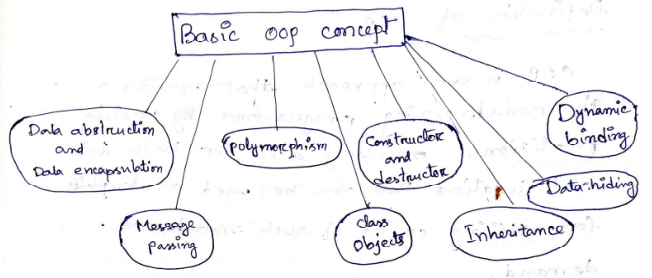
\includegraphics[scale=0.85]{basicoopconcept}
    \section{Features of object oriented paradigm}
      \begin{enumerate}
  
        \item Emphasis on data rather than procedure.
        \item Programms are divided into what are known as objects.
        \item Data structures are designed such that they characterise the object.
        \item Methods that operate on the data of an object are tied togeher in the data structure.
        \item Data is hidden and cannot be accessed by external functions.
        \item Objects may communicae with each other through methods 
        \item New data and methods can be easily added whenever necessary 
        \item Follows bottom up approach in program design
  
      \end{enumerate}
  
    \section{Definaion of OOP}
      \textit{Object Oriented Programming(OOP) is an approach that provides a way of modularizing programmes by creating partitioned memory area for both data and functions that can be used as templates for creating copies of such modules on demand.}
  
    \section{Java History}
      Java is a general purpose OOP language of USA in 1991. Originally called `Oak' by James Gosling, one of the inventors of the language, Java was designed for the development of software for consumer electronic devices like TVs, KCRs, toasters and such other electronic machines. The goal had a strong imapct on the development to make the language simple, portable and highly reliable.
  
      The most striking feature of the language is that it is a "\textit{platform neutral language}". Java is the first programming language that is not tied to any particular hardware or operating system. Programms developed in Java can be executed anywhere on any system.
    
    \section{Java features}
      \begin{itemize}
  
        \item Compiled and interpreted
        \item Platform independent and portable
        \item Object Oriented (pure)
        \item Robust and secure
        \item Distributed:
  
        \begin{itemize}
  
          \item Familiar,
          \item Simple and 
          \item Small
  
        \end{itemize}
  
        \item Multithreaded and interacive
  
        \begin{itemize}
  
          \item High performance
          \item Dynamic and Exensible
          \item Support internet programming (through applet code)
  
        \end{itemize}
  
      \end{itemize}
  
    \section{Java Virtual Machine (JVM) Architecture}
      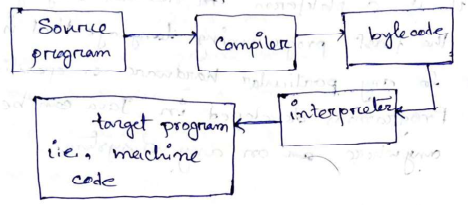
\includegraphics{JVMdiagram}
  
      Normally a computer language is either compiled or interpreted, Java combined both these approaches hus making Java a two stage system. First Java compiler translates source-code into what is known as byte-code instruction. Byte-code are not machine instructions and therefore in the $2^{nd}$ stage
      Java interpreter generates machine code that can be directly executed by the machine that is running the Java program
  
    \section{Platform Independent and Portable}
      The most significant contribution of Java over other programmes can be easily moved from one computer system to another anywhere and anytime.
  
      Changes and upgrades in operating system processors and system resources will not force any changes in Java programmes. This is the reason why Java has become a popular language for programming on internet which interconnects different kinds of system worldwide. We can download a Java applet from a
      remote computer onto our local system via internet and execute it locally.
    
    \section{Java ensures portability in two ways}
      First Java compiler generates byte code instruction that can be implemented on any machine. Secondly the size of the primitive data types are machine independent.
  
    \section{Object-Oriented(pure)}
      Java is a true object-oriented programming language. Almost everything in Java is an object. All programme code and data recide within objects and class.
  
    \section{Robust and Secure}
      Java is a robust language. It provides many safeguard to ensure \ul{reliable code}. It has strict \ul{compile time} and \ul{run-time} checking for data-types. It is designed as a \ul{garbage collected} language relieving the programmer. Virtually all memory management programs. Hava also
      incorporates the concept of exception handling which captures serious errors and eliminate the risk of crashing the system.
  
      Security becomes an important issue for a language that is used for programming an internet. Threat of viruses and abuse of resources are everywhere. Java system also not only verify all memory access but also ensure that no virus are communicated with an applet.
  
    \section{Distributed}
      Java is designed as a distributed language for creating applications on network. It has the ability to share both data and programms. Java application can open and access remote objects on internet as easily as they can do in a local system. This enables multiple programmers at multiple remote
      locations to collaborate and work together on a single project.
  
    \section{Simple, small and familiar}
      Java is a small and simple language. Many features of C and C++ that are either redundant(\textit{duplicate}) or source of unreliable code are not part of Java.
  
      Familiarity is another striking features of Java. To make the language look familiar to the existing programmers, it was modeled on C and C++ language.
  
    \section{Multi-threaded and interactive}
      Multi-threaded means handling mulit-tasks simultaneously. Java supports multi-threaded programmes. This means that we need not wait for the application to finish one task before beginning another.
  
    \section{Dynamic and Extensible}
      Java is a dynamic language. Java is capable of dynamically Linking in new classes, libraries, methods and objects.
  
    \section{High Performance}
     Java performance is impressive for an interpreted language mainly due to the use of intermediate byte-code.
  
    \section{Five Major C++ features that were intentionally removed from Java.}
      Listed below are some major C++ features that were intentionally removed or significantly modified:
  
      \begin{enumerate}
  
        \item Java does not have template classes as in C++
        \item Java does not support multiple inheritance of classes
        \item Java does not support operator overloading
        \item Java does not support global variable
        \item Java does not use pointers.
        \item There are no reader files in Java.
  
      \end{enumerate}
  
    \section{Difference between C and Java}
      Java is a lot like C but the major differences between Java and C is that Java is a object-oriented language and has mechanism to defines classes and objects. In an effort to built a simple and safe language, the Java did not include some of the C features
      
      \begin{enumerate}
  
        \item Java does not include the C unique statements keywords goto, size of and typedef.
        \item Java does not contain the user data types like -- struct, union and enum.
        \item Java does not define the type modifier keywords like auto, extern, register, signed, unsigned.
        \item Java does not have a pre-processor and therefore cannot use \#define, \#include statement.
        \item Java does not support any mechanism for defining variable arguments to functions.
  
      \end{enumerate}
    
    \section{Process of compilation and converting Byte-code into machine code}
      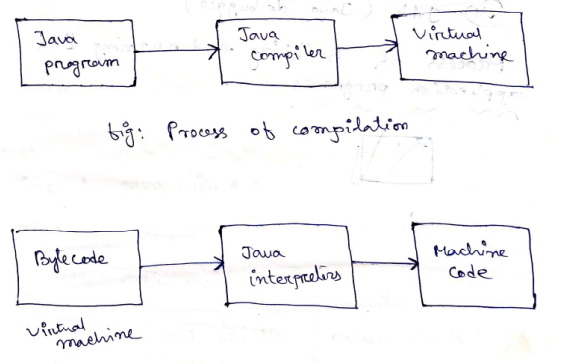
\includegraphics{pocacbcimc}
      
      \begin{center}
        \small \textit{Figure: Process of converting byte-code into machine code.}\normalsize
      \end{center}
  
    \section{Java development Kit (JDK)}
      The Java development kit comes with the collection of tools that are used for developing and running Java Programs. They include:
      
      \begin{enumerate}
  
        \item Appletviewer
        \item Java C (Java Compiler)
        \item Java (Java interpreter)
        \item Java D (Java Disassembler)
        \item Java h (for C header files)
        \item Java doc (for creating HTML documents)
        \item Jdb (Java debugger)
  
      \end{enumerate}
  
    \section{Process of building and running Java application programs}
      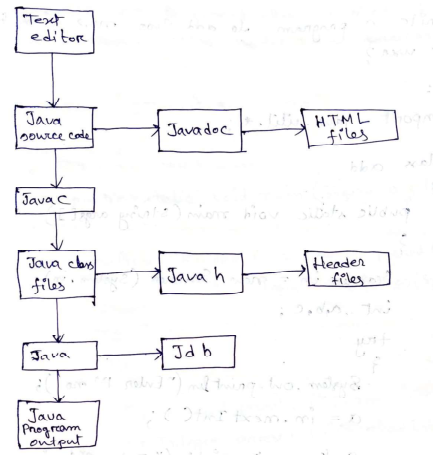
\includegraphics{pobarjap}
    
    \section{Difference between JDK, JRE and JVM}
      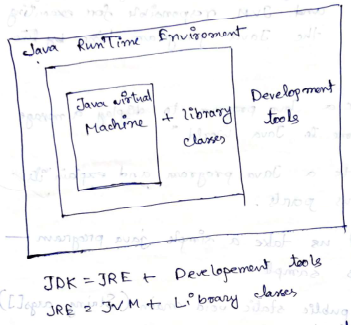
\includegraphics{diffjdkjrejvm}
  
      Let us takes the above diagram to understand the difference between JDK, JRE and JVM
  
    \subsection{JDK}
      JDK provides the environment to develop and execute the Java program. JDK is a kit which includes development tools and JRE.
  
    \subsection{JRE}
      JRE is an installation package which provides environment to only run the Java programming on to our machine JRE is only used by them who only wants to run the Java program and users of our system.
  
    \subsection{JVM}
      JVM is a very important part of both JDK and JRE because it is contained or in-build in both. Whatever Java program we run using JRE or JDK goes into JVM and JVM responsible for executing the Java program line-by-line.
  
    \section{Data-types used in Java}
      Every variable in Java has a data-type. Data-types specifies the size and type of values that can be stored. Java language is rich in its data-types. The varity of data-types available that aloow the programmer to select the type appropriate to the needs of the application.
  
      \includegraphics{pdatatypesJava}
  
    \subsection{Primitive Datatypes (\textit{also called intrinsic or built-in types})}
      Primitive data-types are the basic data-types available within the Java language. There are 8 primitive, viz, boolean, byte, char, short, int, long, float, double. These types serves as building blocks of data manipulation in Java.
  
      The size and range of data types are as follows:
  
      \texttt{byte}$\rightarrow$\texttt{1 bytes}$\rightarrow$\texttt{-128 to +127}
  
      \texttt{short}$\rightarrow$\texttt{2 bytes}$\rightarrow$\texttt{-32768 to +32767}
  
      \texttt{int}$\rightarrow$\texttt{4 bytes}
  
      \texttt{long}$\rightarrow$\texttt{8 bytes}
  
      \texttt{float}$\rightarrow$\texttt{4 bytes}
  
      \texttt{double}$\rightarrow$\texttt{8 bytes}
  
      \texttt{char}$\rightarrow$\texttt{2 bytes}
  
      \texttt{boolean}$\rightarrow$\texttt{1 byte (true/false)}
  
    \section{Control statement in Java}
      Java language processes decision-making capabilities and supports the following statement known as control or decision-making statement
      \subsection{If statement}
  
        The \texttt{if} statement is a powerful decision-making statements and is used to control the following of execution of statement. It is basically a two-way decision statements and is used in conjunction with and expression. It takes the following forms
        \begin{lstlisting}
          if(text expression)
          {
            statement block;
          }
          statement x;
        \end{lstlisting}
  
        \textit{Example}
        \begin{lstlisting}
          .........
          .........
          if(a > 10)
          {
            m = m + 5;
          }
          system.out.println(m);
          .........
          .........
        \end{lstlisting}
  
        \subsection{Switch statement}
        Java has a built-in multiway decision statement known as a switch. The switch statement test the value of a given variable against a list of cause values and when a match is found, a block of statements associates with that case is executed. The general form of the switch statement is as follows
        \begin{lstlisting}
          switch(expression)
          {
            case value_1:
              block_1;
              break;
            case value_2:
              block_2;
              break;
            ........
            ........
            default:
              default_block;
              break;
          }
          statement_x;
        \end{lstlisting}
  
        \subsection{Conditional operator statement}
        Conditional operator is useful for making two way decision. This operator is a combination of `?' and `:' and takes three operands. The general form of conditional statements are as follows
  
        \texttt{conditional expression ? expression 1 : expression 2;}
  
        Conditional expression. Otherwise expression 2 is evaluated, and its value is returned
  
        \textit{Example}
        \begin{lstlisting}
          if(x < 0)
            flag = 0;
          else
            flag = 1;
        \end{lstlisting}
        can be written as 
        \begin{lstlisting}
          flag = (x < 0) ? 0 : 1;
        \end{lstlisting}
  
    \section{Looping statement in Java}
      In looping a sequence of statement are executed until some condition for the termination of the loop are satisfied. Depending on the position of the control statement on the loop, a control structure may be classified either as the entry control loop or an exit control loop. Java language provides
      three contruct for performing loop operation. They are
  
      \subsection{While statement}
        The simplest of all the looping stature of Java in the while statement. The basic formal of the while statement is 
        \begin{lstlisting}
          Initialisation;
          while(test condition)
          {
            body of the loop;
          }
        \end{lstlisting}
        The while is an entry control loop statement. The test condition is evaluated and if the condition is true, then the body of loop is executed.
        
        \textit{Example}
        \begin{lstlisting}
          .............
          .............
          i = 1;
          while(i < 10)
          {
            System.out.println("i=" + 1);
            i = i + 1;
          }
          .............
          .............
        \end{lstlisting}
      
      
      \subsection{The do-while loop}
        The do-while statement is a exit control loop (\textit{The body of the loop executed at-least once if condition fails}). Since the test condition is evaluated at the bottom of the loop the do-while construct and provides an exit control loop and therefore the body of the loop is always executed at-least once. It takes the following form:
  
        \begin{lstlisting}
          Initialisation;
          do 
          {
            Body of the loop;
          } while(test condition);
        \end{lstlisting}
        
        \textit{Example}
        \begin{lstlisting}
          .............
          .............
          i = 1;
          do 
          {
            System.out.println("i=" + i);
            i = i + 1;
          } while(i < 10);
          .............
          .............
        \end{lstlisting}
      
      \subsection{The for statement}
        The for loop is another entry control loop that provides a more concise loop control structure. The general form of the for loop is
        
        \begin{lstlisting}
          for(initialisation; test condition; increment)
          {
            Body of the loop;
          }
        \end{lstlisting}
    
    \section{Arrays in Java}
      An array is a group of contiguous or related data items that share a common name. In Java, array can be declared as
      
      \begin{lstlisting}
        type arrayname[];
        \end{lstlisting}
        or 
        \begin{lstlisting}
        type[] arrayname;
      \end{lstlisting}
      
      \textit{Example}
      \begin{lstlisting}
        int n[];
        float a[];
      \end{lstlisting}
      
      In Java we do not enter the size of the array in declaration.
      
      In Java, array can be created as follows 
      
      \texttt{array name = newtype[size];}
      
      \textit{Example}
      
      \begin{lstlisting}
        n = newint[8];
        a = newfloat[10];
      \end{lstlisting}
      
      Array can be initialized as follows
      
      \texttt{type arrayname[] = { list of values };}
      
      \textit{Example}
      
      \begin{lstlisting}
        int n[] = { 35, 10, 12, 55 };
      \end{lstlisting}
    
    \section{For-each statement}
      The Java `for-each' loop or enhanced for loop provides an alternative approach to traverse the array or collection in Java. It is mainly used to traverse the array or collection elements. The advantages of for-each loop is that it eliminates the posibility of bugs and makes the code more readable.
      It is known as the for each loop beacuse it traverses each element one by one. The syntax of Java for-each loop consists of data-type with the variable followed by a colon(:) then array or collection
      \begin{lstlisting}
        for(data-type: array/collection)
        {
          // body of for-each loop;
        }
      \end{lstlisting}
  
      \emph{Example}
      
      \begin{lstlisting}
        class forEachLoop{  
          public static void main(String args[]){  
            //declaring an array  
            int arr[]={12,13,14,44};  
            //traversing the array with for-each loop  
            for(int i:arr){  
              System.out.println(i);  
            }
          }
        }
      \end{lstlisting}
    
    \section{Tokens}
      Java includes five types of token, they are:
  
      \begin{itemize}
  
        \item Reserve keyword
        \item Identifiers
        \item Literals
        \item Operators
        \item Seperators(\texttt{; () ,})
  
      \end{itemize}
  
      Token is an individual unit of a program
    
    \section{Java Constant}
      The syntax to declare a constant is as follows:
      \begin{lstlisting}
        static final datatype identifier_name=value;
      \end{lstlisting}
      For example, price is a variable that we want to make constant.
      
      \texttt{static final double PRICE=432.78;}
      
      In Java, to declare any variable as constant, we use static and final modifiers.
    
    \section{Java Variables}
      A variable is a container which holds the value while the Java program is executed. A variable is assigned with a data type.
      
      There are three types of variables in Java:
  
      \begin{enumerate}
  
        \item Local variable\\
          A variable declared inside the body of the method is called local variable.
      
        \item Instance variable\\
          A variable declared inside the class but outside the body of the method, is called an instance variable.
      
        \item Static variable\\
          A variable that is declared as static is called a static variable. It cannot be local.
  
      \end{enumerate}
      
      \textit{Example}
      \begin{lstlisting}
        public class A  
        {  
            static int m=100;//static variable  
            void method()  
            {    
                int n=90;//local variable    
            }  
            public static void main(String args[])  
            {  
                int data=50;//instance variable    
            }  
        }
      \end{lstlisting}
    
    \section{Java Expressions}
      A Java expression consists of variables, operators, literals, and method calls.
      
      \textit{Example}
      
      \texttt{int score;}
      
      \texttt{score = 90;}
      
      Here, \texttt{score = 90} is an expression that returns an \texttt{int}. Consider another example,
      
      Double \texttt{a = 2.2, b = 3.4,} result;
      
      \texttt{result = a + b - 3.4;}
      
      Here, \texttt{a + b - 3.4} is an expression.
      
      
      \subsection{Relational Expression}
        A relational-expression indicates the condition that the system evaluates.
        
        The Syntax is \texttt{variable1 relation\_operator variable2;}
        
        \textit{Example}
        
        \texttt{var1 == var2}
        \texttt{var1 > var2}
      
      \subsection{Logical Expression}
        A logical expression is a statement that can either be true or false.
        
        The Syntax is \texttt{condition1 \&\& condition2}
        
        \texttt{if(condition1 \&\& condition2)}
        
        \texttt{d = a + b + c}
        
        \textit{Example}
        \begin{lstlisting}
        if ((a < b) && (b == c)) {
          d = a + b + c;
          System.out.println("The sum is: " + d);
        }
        \end{lstlisting}
      
      \subsection{Boolean Expression}
        A boolean expression is a Java expression that returns a boolean value: true or false.
        
        This is useful when we want to compare values to find answers.
        
        \textit{Example}
        \begin{lstlisting}
        int x = 10;
        int y = 9;
        System.out.println(x > y); // returns true, because 10 is higher than 9
        \end{lstlisting}
    
    \section{Java Operators}
      Following are the list of Java operators:
      
      \resizebox{\columnwidth}{!}{%
      \begin{tabular}{|l|l|l|l|}
      \hline
      \textbf{Operator}          & \textbf{Name}       & \textbf{Description}                                                    & \textbf{Example}          \\ \hline
      \texttt{+}                 & Addition            & Adds together two values                                                & \texttt{x+y}              \\ \hline
      \texttt{-}                 & Subtraction         & Subtracts one value from another                                        & \texttt{x-y}              \\ \hline
      \texttt{*}                 & Multiplication      & Multiplies two values                                                   & \texttt{x*y}              \\ \hline
      \texttt{/}                 & Division            & Divides one value by another                                            & \texttt{x/y}              \\ \hline
      \texttt{\%}                & Modulus             & Return the division remainder                                           & \texttt{x\%y}             \\ \hline
      \texttt{++}                & Increment           & Increases the value of a variable by 1                                  & \texttt{++x}              \\ \hline
      \texttt{--}                & Decrement           & Decreases the value of a variable by 1                                  & \texttt{--x}              \\ \hline
      \texttt{=}                 & Assignment          & Assigns a value to a variable                                           & \texttt{x=10}             \\ \hline
      \texttt{+=}                & Addition assignment & Adds certain value to itself and assigns the total value back to itself & \texttt{x+=10}            \\ \hline
      \texttt{==,>,<,>=,<=}      & Comparison          & Compares two values                                                     & \texttt{x==10, x>10, etc} \\ \hline
      \texttt{\&\&,||,!}         & Logical             & Applies logic                                                           & \texttt{x \&\& y,etc}     \\ \hline
      \end{tabular}%
      }
    
    \pagebreak
    \section{Questions}
    % UNANSWERD QUESTIONS
    % \subsection{Why is Java known as platform-neutral language?}
    % \subsection{How is Java more secured than other languages?}
    % \subsection{What is multi-threading? How does it improve the performance of Java?}
    % \subsection{What is Java? or Why Java?}
    % \subsection{Explain different features of Java}
    % \subsection{What is JDK and JRE? What is the difference between these two?}
    % \subsection{Explain the process of building and running Java application programs}
    % \subsection{Write a Java Program to display a message "Welcome to Java World"}
    % \subsection{Difference between C++ and Java?}
    % \subsection{Type Casting in Java? Explain with example}
    % \subsection{Major features of Java}
    
    \subsection{How is Java strongly associated with the internet?}
      Java is strongly associated with the internet because of the fact the first application programme written in Java was `Hot Java', a web browser to run applet on internet. Internet users can use Java to create applet programme and run then locally using a Java, enabled browser such as `Hot Java'.
      They can also use a Java enabled browser to download an applet located on a computer anywhere in the internet and run it on his local computer. That is why Java is popularly known as Internet language.
  
      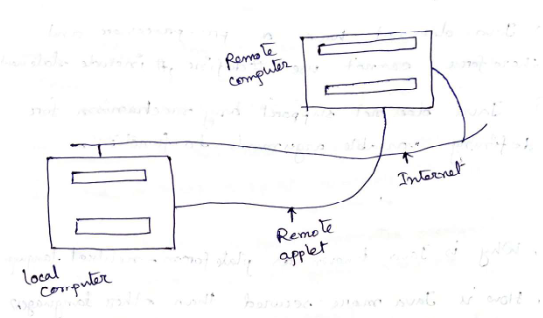
\includegraphics{q4diagram1}
  
      \begin{center}
        \small \textit{Figure: Download of applets via internet}\normalsize 
      \end{center}
    
    \subsection{How is world wide web? What is the contribution of Java to the world web?}
      World wide web is an open information retrival system designed to be used in the internets distributed environment. This system contains what are known as webpage that provide both information and controls. This is made possible with the help of a language called \textbf{Hyper Text Markup Lanague
      (HTML)}. Web pages contains HTML tags that enable us to find retrieve, manipulate and display documents world wide. Java was meant to be used in distributed environment just as internet. Since both the web and Java share same philosophy, Java communicates with a web page through a special tag
      called <APPLET>
    
    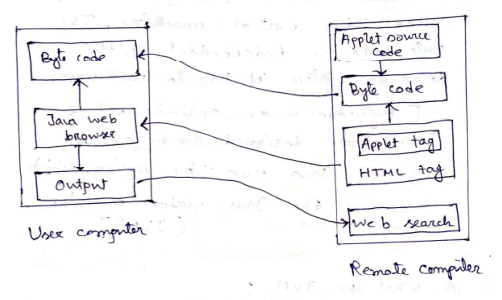
\includegraphics{q5diagram}
      
    \subsection{Describe the various system required for internet programming?}
      Following are the different system required for internet programming:
  
      \begin{enumerate}
  
        \item Internet Connection
        \item Webserver
        \item HTML
        \item APPLET tag
        \item Java Code
        \item Byte Code
        \item Proxy Server
        \item Mail Server
  
      \end{enumerate}
    
    \subsection{What is `Byte-code'?}
      The Java Byte-code is a machine instruction for a Java Processor chip called Java Virtual Machine. The byte-code is independent of the computer system it has to run upon.
    
      [ Byte-code is an optimise set of instructions designed to be executed by the Java run time system, which is called the Java Virtual Machine (JVM) ]
    
    \subsection{What is JVM?}
      Programmes written in Java are compiled into Java byte-code which is then interpreted by a special Java interpreter for a specific platform. Actually this Java interpreter is known as the Java Virtual Machine (JVM). This machine is called Byte-code. Actually the Java interpreter running on any
      machine appears and behaves like a virtual processor chip, that is why -- Java Virtual Machine.
    
    \subsection{What is Java API?}
      The Java API(Application Programme Interface) are libraries of compiled code that can be used in a programme. In otherwords, the Java API consists of the function and variables that programme are allowed to use their applications.
    
    \subsection{Write a Java program to display `Hello World'}
    
      \begin{lstlisting}
        import Java.io.*;
        
        class show
        {
          public static void main(string args[])
          {
            system.out.println("Hello World");
          }
        }
      \end{lstlisting}
    
    \subsection{Write a program to add two numbers given by the user.}
      \begin{lstlisting}
        import Java.util.*;
      
        class add
        {
          public static void main(string args[])
          {
            scanner in = new scanner(system.in);
            int a,b,c;
            try
            {
              system.out.println("Enter 1st number: ");
              a = in.nextInt();
              system.out.println("Enter 2nd number: ");
              b = in.nextInt();
              c = a + b;
              system.out.println("The result is " +c);
            }
            catch(Exception e)
            { }
          }
        }
      \end{lstlisting}
    
    \subsection{Write a Java program to convert the temperature from Fahrenheit to Celsius?}
      \begin{lstlisting}
        import Java.util.*;
        
        class temp 
        {
          public static void main(string args[])
          {
            double a,b;
            char c; scanner in=newScanner(system.in);
            try
            {
              do 
              {
                System.out.println("Enter the temperature: ");
                a = in.nextDouble();
                b = ((a-32)/1.8);
                System.out.println(a+"*F'="+b"*c");
                System.out.println("Do you want to continue");
                c = in.next().charAt(0);
              } while(c=='y');
            }
          }
        }
      \end{lstlisting}
    
    \subsection{What is JRE(Java Runtime Environment)?}
      JRE stands for Java Runtime Environment and may also be written as Java RTE. The Java Runtime Environment provides the minimum requirement for executing the Java application, it consists of the Java Virtual Machine(JVM), core classes and supporting files.
    
    
    \subsection{Write a Java Program and explain its various parts.}
      Let us take a simple Java program:
    
      \begin{lstlisting}
        class sample
        {
          public static void main(String args[])
          {
            System.out.println("Java is better than C++");
          }
        }
      \end{lstlisting}
      \textit{Explanation}
  
      The first line `class sample' declares a class which is an object-oriented construct. Java is a true OOP language therefore everything must be placed inside a class. `class' is a keyword and `sample' is a Java identifier that specifies the name of the class.
      
      Every class defination in Java begins with an opening braces (\{) and end with a matching closing braces (\}).
      \ \\
      
      The third line
      
      \large \texttt{\textbf{Public static void main(String args[])}}\normalsize defines a method named main. Every Java application program must include the main method. This is the starting point for the interpreter to being the execution of the program. This line contains a number of keyword viz,
      \texttt{public}, \texttt{static} and \texttt{void}.
      
      \large \texttt{\textbf{public}}\normalsize: The keyword `\texttt{public}' is an access specifier that declares the main method as unprotected and therefore making it accessible to all other class.
      
      \large \texttt{\textbf{static}}\normalsize: Next appears the keywords `\texttt{static}' which declares this method as one that belongs to the entire class and not a part of any object of the class.
      
      \large \texttt{\textbf{void}}\normalsize: The type modifier `\texttt{void}' states that the main method does not  return any value.
      
      \ \\
      The only executable statement in the program is 
      
      \large \texttt{\textbf{System.out.println("Java is better than C++");}}\normalsize 
      
      The `\texttt{println}' method is a member of `\texttt{out}' object which is a static data member of system class.
    
    
    \subsection{Explain \texttt{public static void main(sting args[])}}
      By Default in Java main method accepts command line argument `\texttt{args}' is decleared as an array of strings known as string object. Any arguments provided in the command line are passed to the array `\texttt{args}' as its elements.
      
      \ \ \ \ \ \ \ \ \ \ \ \ \ \ \ \ \ \ \ \ \ \ \ \ \ \texttt{arg[0]}\ \ \ \ \texttt{arg[1]}\ \texttt{arg[2]} \texttt{arg[3]}
      
      \Large \texttt{C:\textbackslash JavaPrg> \small Basic | Fortran | C\ \ \ \ | C++}\normalsize
      
      The above command line include four arguments.
    
    \subsection{Write a Java program using command line argument and explain its various parts}
      \begin{lstlisting}
        class continueTest
        {
          public static void main(string args[])
          {
            int count, i = 0;
            string str;
            count=args.length;
            System.out.println("Number of arguments" + count);
            while(i < count)
            {
              str = args[i];
              i = i+1;
              System.out.println(i+":"+"Java is"+str);
            }
          }
        }
      \end{lstlisting}
      
      The above program illustrate the use of command line argument compile and run the program with the command line as follows:
      
      \Large \texttt{C:\textbackslash JavaPrg>} \small Java C comline. Test secure, Rebust, compile, interpreted distributed Multi-threaded\normalsize
      
      \noindent \emph{Number of arguments = 6}
  
      \begin{enumerate}

        \item Java is secured
        \item Java is robust
        \item Java is compiled
        \item Java is interpreted
        \item Java is distributed
        \item Java is multi-threaded
  
       \end{enumerate}
    
      
    \subsection{What is Java IDE? List two IDE for Java}
      A Java IDE (\textit{Integrated Development Environment}) is a software application which enable user to more easily write and debug Java program, many IDEs provides features like syntax highlighting and code completion which help the user to code move easily.
    
      Two popular IDE for Java are as follows:
  
      \begin{itemize}
  
        \item \underline{Eclipse}: Eclipse is a FOSS IDE, plus a developer tool framework that can be extended for a particular development need.
        \item \underline{Netbeans}: The Netbeans IDE is a also a free and open source IDE for software developers. We can easily create Java application for mobile devices.
  
      \end{itemize}
    
    \subsection{Write down the difference between}
      \subsubsection{Integer and Floating point datatype}
        \resizebox{\columnwidth}{!}{%
        \begin{tabular}{|l|l|}
        \hline
        \multicolumn{1}{|c|}{\textbf{Integer datatype}} &
          \multicolumn{1}{c|}{\textbf{Floating Point datatype}} \\ \hline
        \begin{tabular}[c]{@{}l@{}}Integer datatype can hold \\ whole numbers.\end{tabular} &
          \begin{tabular}[c]{@{}l@{}}Floating point datatype holds num-\\ bers containing fractional part.\end{tabular} \\ \hline
        \begin{tabular}[c]{@{}l@{}}Java supports 4types of inte-\\ gers such as byte, short, int, long.\end{tabular} &
          \begin{tabular}[c]{@{}l@{}}There are two kind of floating point\\ storage in Java viz floating and double.\end{tabular} \\ \hline
        \end{tabular}%
        }
      
      \subsubsection{Character and Boolean datatype}
        \resizebox{\columnwidth}{!}{%
        \begin{tabular}{|l|l|}
        \hline
        \multicolumn{1}{|c|}{\textbf{Character datatype}} &
          \multicolumn{1}{c|}{\textbf{Boolean datatype}} \\ \hline
        \begin{tabular}[c]{@{}l@{}}In order to store character constant in \\ memory, Java provides a character datatype \\ called char.\end{tabular} &
          \begin{tabular}[c]{@{}l@{}}Boolean type is used when we want to test a \\ particular condition during the execution of \\ the program.\end{tabular} \\ \hline
        \begin{tabular}[c]{@{}l@{}}The size of char type is 8 bytes but basically\\  it can hold only a single character\end{tabular} &
          \begin{tabular}[c]{@{}l@{}}There are only two values that a boolean type \\ can take -- true or false\end{tabular} \\ \hline
        \end{tabular}%
        }

    \subsection{Explain the term -- Casting, Automatic type conversion}
      \subsubsection{Casting}
        We often encounter situation where there is a need to store a value of one type into, a variable of another type. In such situation we must cast the value to be stored by preceding it with the type name with parenthesis. The syntax is:

        \begin{lstlisting}
          Type variable 1 = (type) variable 2;
        \end{lstlisting}

        The process of converting one datatype to another is called casting 

        \textit{Example}:

        \begin{lstlisting}
          int m = 50;
          byte n = (byte)m;
        \end{lstlisting}

      \subsubsection{Automatic type conversion}
        For some time it is possible to assign a value of one type to a variable of a different type without a cast. Java does the conversion of the assigned value automatically, this is known as automatic type conversion. Automatic  type conversion is possible only if the destination type has enough
        precision to store the source value.

        \textit{Example}

        \texttt{int is large enough to hold a byte value }

        \texttt{byte b = 75;}

        \texttt{int a = b;}

        \texttt{are valid declaration}

    \subsection{How main function is defined in Java?}
      In Java \texttt{main()} function can be defined within a class definition. The syntax is as follows

      \begin{lstlisting}
        class FstJava
        {
          public static void main(string args[])
          {
            System.out.println("Hellow Java");
          }
         }
      \end{lstlisting}
  
      Here \texttt{public static void main (string args[])} defines a method\dots\dots system class%}}}

            \chapter{Unit 2}%{{{
  \section{Polymorphism in Java.}
  Polymorphism in Java is a concept by which we can perform a
  single action in different ways.

  There are two types of polymorphism in Java: compile-time 
  polymorphism and runtime polymorphism. We can perform 
  polymorphism in Java by method overloading and method 
  overriding.

  \section{Inheritance in Java}
  \begin{lstlisting}
    class A_class {
      void disp_A () {
        System.out.println("Display Grandparent");
      }
    }
    class B_class {
      void disp_B () {
        System.out.println("Display Parent");
      }
    }
    class C_class {
      void disp_C () {
        System.out.println("Display child");
      }
    }
    
    public class multilvl {
      public static void main(String[] args) {
        C_class c = new C_class();
        c.disp_A();
        c.disp_B();
        c.disp_C();
      }
    }
  \end{lstlisting}
  \section{Packages in Java}

  \section{Interface}
  An interface is basically a type of class like classes, interface contains methods and variables
  but with a mahor difference. The difference is that interface defines only abstruct method and final fields. This means that interfaces dpnpt specify any code to implement these methods and daya fields contains only constants. Therefore it is the responsibility of the class that impliments and
  interface to define the code for implementation of these methods.

  The syntax for defining and interface is very similar to that for defining a class. The general form of interface declaration is -

  \begin{lstlisting}
    interface InterfaceName {
      variable declearation;
      method declearation;
    }
  \end{lstlisting}
  Here `interface' is a keyword and `InterfaceName' is any varid Java variable.

  Now variables are declared as follows - 
  \begin{lstlisting}
    static final type VariableName = value;
  \end{lstlisting}
  and the method can be declared as -
  \begin{lstlisting}
    returntype methodName(parameter_list);
  \end{lstlisting}

  \emph{Example}
  \begin{lstlisting}
    interface item {
      static final int code = 1001;
      static final string name = "Java";
      void display();
    }
  \end{lstlisting}

  \newpage

  \section{Questions}
  \subsection{Why Multiple inheritance is not supported in Java}
  \subsection{What is class in Java? How to define the class 
  in Java? Give its syntax.}
  \subsection{What is object? How to instentiate and create 
  the object?}
  We can pass objects as arguments in Java. The following 
  program demonstrates how to pass and return objects in Java.
  \begin{lstlisting}
    class obj {
      int a;
      void get_a() {
        a=10;
      }
      obj calc(obj m){ //object as argument {
        obj x=new obj();
        x.a=m.a;
        return x; //returning object
      }
      void put_a() {
        System.out.pintln("a="+a);
      }
    }

    public class objectPassing {
      public static void main(String[] args)
        {
        obj o=new obj();
        o.get_a();
        System.out.println("Value of o object");
        o.put_a();
        obj o1=new obj();
        o1=o1.calc(o);
        System.out.println("Value of o1 object");
        o1.put_a();
      }
    }
  \end{lstlisting}


  \subsubsection{Passing objects to a constructor}
  \begin{lstlisting}
    class covld 
    {
      int a;
      covld(int x)
      {
          a=x;
        }
      covld(covld m, covld n)
      {
          int h;
          h=m.a+n.a;
          System.out.println("The result is "+h);
        }
    }

    /**
     * contruc_obj
     */
    public class contruc_obj {

      public static void main(String[] args) {
        covld a1=new covld(12);
        covld a2=new covld(13);
        covld a3=new covld(a1, a2);
      }
    }
  \end{lstlisting}

  \subsection{What is constructor in Java? How constructors are defined in Java?}
  \subsection{How objects are destroyed in Java}
 
  \subsection{Method overloading / overwritting (one-line definition)(Difference)(give two examples.)}
  \subsection{Finalize method and garbage collection method.}
  \subsection{\texttt{Finalize()} method in Java and how to use.}%}}}
 
\newpage
\section{How to implement package in Java}
\begin{itemize}
  \item First we create a package named empPack (\textit{say})
  \item Create class file ie create a Java file test, test1 (\textit{say})
\begin{lstlisting}
  package empPack;

  class test {
    public void disp_test() {
      System.out.println("Hello display test ");
    }
  }
  public class test1 extends test {
    public void disp_test1() {
      System.out.println("Hello display test 1");
    }
  }
\end{lstlisting}
  \item Now again create a Java file having main method where we will import the above package
\begin{lstlisting}
  import empPack.*;
  public class packtest22 {
    public static void main(String[] args) {
      test1 t=new test1();
      t.disp_test();
      t.disp_test1();
    }
  }
\end{lstlisting}
\end{itemize}

\chapter{Unit 3}
\section{What is thread?}
\subsection{How to create a thread in java? Explain with example.}
\subsection{Thread and runnable difference}
\section{Exceptions Handling}
\subsection{What is java exception? How exceptions are handled in Java? List down some pre-defined java exceptions.}

\chapter{Unit 5}
\section{JDbC}
\subsection{Maintask of JDbC}
\subsection{Applications}
\subsection{JDbC Architecture}
\subsection{Different components of JDbC}
\subsection{Different JDbC Driver}
\subsection{How database connection can be established through JDbC (\emph{extablishing connectivity and working with connection interfaces})}
\subsection{How can we create and execute SQL statements in JDbC. Explain with example}
\subsection{How to work with result set objects? Give examples}



% }}}
\end{document}
